\documentclass[]{article}
\usepackage{amsmath}\usepackage{amsfonts}
\usepackage[margin=1in,footskip=0.25in]{geometry}
\usepackage{mathtools}
\usepackage{hyperref}
\hypersetup{
    colorlinks=true,
    linkcolor=blue,
    filecolor=magenta,
    urlcolor=cyan,
}
\usepackage[final]{graphicx}
\usepackage{listings}
\usepackage{courier}
\lstset{basicstyle=\footnotesize\ttfamily,breaklines=true}

% \usepackage{wrapfig}
\graphicspath{{.}}

\begin{document}
\hspace{-1.8em}
Name: Hongda Li
\\
Class: CSE 546
\section*{1. Probability and Statistics}
    \subsection*{(A.1)}
        Given the test is positive, what is the probability that I have the disease? It's equivalent to, among all 10k people who tested positive, what is the probability of them actually having the disease? (Using Bayes Theorem, I used 10k people but the sample size doesn't matter they cancel out in the numerator and denominator)
        $$
        \frac{1}{(1\times 0.99) + (9999\times 0.01)} \approx 0.009
        $$
    \subsection*{(A.2)}
        \subsubsection*{(A.2.a)}
            \textbf{Claim a1.2..0} We need the statement that: $\mathbb{E}\left[XY\right] = \mathbb{E}\left[X^2\right]$ to build up to the solution. Staring with the definition we have: 

            \begin{align*}\tag{1.2.a.1}\label{eqn:1.2.a.1}
                \mathbb{E}\left[XY\right] = 
                &\sum_{x\in\Omega_X}^{}
                    \sum_{y\in\Omega_Y}^{}
                        xy \mathbb{P}\left(X = x \cap Y = y\right)
                \\
                =&\sum_{x\in\Omega_X}^{}
                    \sum_{y\in\Omega_Y}^{}
                        xy \mathbb{P}\left(Y = y|X = x\right)\mathbb{P}\left(X = x\right)
                \\
                =&  \sum_{x\in\Omega_X}^{}
                    x \mathbb{P}\left(X = x\right)
                        \underbrace{
                            \sum_{y\in\Omega_y}^{}
                            y \mathbb{P}\left(Y = y|X = x\right)
                        }_
                        {=\mathbb{E}\left[Y| X = x\right] = x}
                \\
                =&  \sum_{x\in\Omega_X}^{}
                    x^2 \mathbb{P}\left(X = x\right)
                \\
                =& \mathbb{E}\left[X^2\right]
            \end{align*}
            Then, following the same step as in \hyperref[eqn:1.2.b.1]{1.2.b.2} but this time we are replacing $\mathbb{E}\left[X\right]\mathbb{E}\left[Y\right]$ with value gotten from \hyperref[eqn:1.2.a.1]{1.2.a.1}, we will have: 
            \begin{align*}\tag{1.2.a.2}\label{eqn:1.2.a.2}
                \text{Cov}(X, Y) =& \mathbb{E}\left[(X - \mathbb{E}\left[X\right])
                    ( Y - \mathbb{E}\left[Y\right])
                \right]
                \\
                =& 
                \mathbb{E}\left[XY\right] - \mathbb{E}\left[X\right]^2
                \\
                =&
                \underbrace
                {\mathbb{E}\left[X^2\right] - \mathbb{E}\left[X\right]^2}_
                {\text{Just the variance}}
                \\
                =&
                \mathbb{E}\left[(X - \mathbb{E}\left[X\right])^2\right]
            \end{align*}

        \subsubsection*{(A.2.b)}
            If rvs $X,Y$ are independent to each others, then: 
            \begin{equation*}\tag{1.2.b.1}\label{eqn:1.2.b.1}
                \mathbb{E}\left[XY\right] = \mathbb{E}\left[X\right]\mathbb{E}\left[Y\right]
            \end{equation*}
            Therefore, starting with the definition of Covariance, we have: 

            

            \begin{align*}\tag{1.2.b.2}\label{eqn:1.2.b.2}
                &\mathbb{E}\left[( X- \mathbb{E}\left[X\right])
                    (X - \mathbb{E}\left[Y\right])
                \right]
                \\
                =&
                \mathbb{E}\left[XY - 
                    X \mathbb{E}\left[Y\right]
                    -Y \mathbb{E}\left[X\right]
                \right]
                +
                \mathbb{E}\left[X\right]\mathbb{E}\left[Y\right]
                \\
                =&
                \mathbb{E}\left[XY\right] - 2 \mathbb{E}\left[X\right]\mathbb{E}\left[Y\right]
                + 
                \mathbb{E}\left[X\right]\mathbb{E}\left[Y\right]
                \\
                =&
                \mathbb{E}\left[X\right]\mathbb{E}\left[Y\right] - 2 \mathbb{E}\left[X\right]\mathbb{E}\left[Y\right]
                + 
                \mathbb{E}\left[X\right]\mathbb{E}\left[Y\right]
                \\
                =& 0
            \end{align*}
            From the second step to he third step, linearity property of the expected value for random variable is used to factor out the constant value out of the expected value operator. 
    \subsection*{(A.3)}
        $X, Y$ are independent rvs and has $f,g$ as their PDF, $h$ is the PDF for random variable $Z:= X + Y$. 
        \subsubsection*{(A.3.a)}
            \textbf{Objective: } Figure out a PDF for rv $Z$. By Definition, we have: 
            \begin{align*}\tag{1.3.a.1}\label{eqn:1.3.a.1}
                h(z) &= \mathbb{P}\left(Z = z\right)
                \\
                =& 
                \mathbb{P}\left(X + y = z\right)
                \\
                =&
                \int_{-\infty}^{\infty} 
                    \mathbb{P}\left(Y = z - x|X = x\right)
                    \mathbb{P}\left(X = x\right) 
                dx
                \\
                =& 
                \int_{-\infty}^{\infty} 
                    \mathbb{P}\left(Y = z - x\right)
                    \mathbb{P}\left(X = x\right) 
                dx \quad \text{By Independence assumption}
                \\
                =& 
                \int_{-\infty}^{\infty} g(z - x)f(x)dx
            \end{align*}
        \subsubsection*{(A.3.b)}
            \textbf{Objective: } Assume that, $X,Y$ are unif random on $[0, 1]$, Find PDF for rv $Z$. 
            \\
            Take note that, since $Z = X + Y$, and $X, Y\in [0, 1]$ then $Z \in [0, 2]$, so the integral we are trying to solve will be: 
            \begin{equation*}\tag{1.3.b.1}\label{eqn:1.3.b.1}
                \int_{0}^{1} f(x)g(z - x)dx
            \end{equation*}
            The idea is convolution, we are sliding 2 square across each other, $z$ controls the displacement of the block on the left, the started just touching each other, and then slides all the way until the block leaves each other. The area that they overlaps with each other is just: 
            \begin{equation*}\tag{1.3.b.2}\label{eqn:1.3.b.2}
                \int_{0}^{\max(z, 2 - z)}dx
                =
                \begin{cases}
                    z & z\in [0, 1]
                    \\
                    2 - z & z\in (1, 2]
                    \\
                    0 & \text{else}
                \end{cases}
            \end{equation*}
            So it's just an triangle. 
    \subsection*{(A.4)}
        This just standardization, given variable $X\sim \mathcal{N}(\mu, \sigma^2)$, the standardize variable $Z$ with $\mathcal{N}(0, 1)$ will be given as: 
        \begin{equation*}\tag{1.4.1}\label{eqn:1.4.1}
            Z = \frac{x - \mu}{\sigma}
        \end{equation*}
        This can be shown by considering the CDF for the normal distribution $\Phi$, and it's going to look like: 
        \begin{align*}\tag{1.4.2}\label{eqn:1.4.2}
            \mathbb{P}\left(X \le a\right)
            =&
            \int_{-\infty}^{a} 
                \frac{1}{\sigma \sqrt{2\pi}} 
                \exp \left(
                    \frac{-1}{2}
                    \left(
                        \frac{x -\mu}{\sigma}
                    \right)^2
                \right)
            dx
            \\
            =& 
            \int_{x = -\infty}^{x = a} 
                \frac{1}{\sigma \sqrt{2\pi}}
                \exp\left(
                    \frac{-z^2}{2}
                \right)
            \sigma dz \quad \text{Sub: } z = \frac{x - \mu}{\sigma}
            \\
            =&
            \int_{x = -\infty}^{x = a} 
                \frac{1}{\sqrt{2\pi}}
                \exp\left(
                    \frac{-z^2}{2}
                \right)
            dz \quad
        \end{align*}
        Variable $z$ has standard normal distribution because the Integrand inside is a standard normal distribution. Therefore, we can conclude that $a = \frac{1}{\sigma}, b = -\frac{\mu}{\sigma}$. 
    \subsection*{(A.5)}
        $X_n$ where $1 \le n \le n$ are idd rvs, each with mean $\mu$ and variance of $\sigma^2$, define $\hat{\mu}_n = \frac{1}{n}\sum_{i = 1}^n X_i$, what is the mean and variance of $\sqrt{n}(\hat{\mu}_n - \mu)$? 
        Firstly, we want to show the expected value of $\hat{\mu}_n$ is $\mu$: 
        \begin{align*}\tag{1.5.1}\label{eqn:1.5.1}
            &\mathbb{E}\left[
                \frac{1}{n} \sum_{i = 1}^{n} X_i
                \right]
            \\
            =& \frac{1}{n}\mathbb{E}\left[
                \sum_{i = 1}^{n}X_i
            \right]
            \\
            =&
            \frac{1}{n}n\mu = \mu
        \end{align*}
        So then: 
        \begin{align*}\tag{1.5.2}\label{eqn:1.5.2}
            \mathbb{E}\left[\sqrt{n}(\hat{\mu}_n - \mu)\right]
            =&
            \sqrt{n}\mathbb{E}\left[\hat{\mu}_n - \mu\right]
            \\
            =& \sqrt{n}(\mu - \mu) = 0
        \end{align*}
        \\
        The variance of the expression cen be figured out as: 
        \begin{align*}\tag{1.5.3}\label{eqn:1.5.3}
            \text{Var}\left[\sqrt{n}\hat{\mu}_n - \sqrt{n}\mu\right]
            =& n \text{Var}\left[\hat{\mu}_n\right]
            \\
            =&
            \frac{1}{n} \text{Var}\left[
                \sum_{i =1 }^{n}X_i
            \right] 
            \\
            =& \frac{1}{n}\sum_{i = 1}^{n}\text{Var}\left[X_i\right]
            \\
            =&  \frac{n}{n}\sigma^2
            \\
            =& \sigma^2
        \end{align*}
    \subsection*{(A.6)}
        \subsubsection*{(A.6.a)}
            The key is to use the fact that $X_i$ are idd rvs, and starting with the definition of $\hat{F}_n(x)$, we have: 
            \begin{align*}\tag{1.6.a.1}\label{eqn:1.6.a.1}
                \mathbb{E}\left[\hat{F}_n(x)
                    \right] =&
                    \mathbb{E}\left[
                        \frac{1}{n}\sum_{i = 1}^{n}\mathbf{1}\{X_i \le x\}
                    \right]
                \\
                =&
                \frac{1}{n}
                    \sum_{i = 1}^{n}
                        \mathbb{E}\left[\mathbf{1}\{X_i\le x\}\right]
                \\
                =& 
                \frac{1}{n} \sum_{i =1}^{n}F(x)
                \\
                =& F(x)
            \end{align*}
            From the first step to the second step, we use the assumption that $X_i$ are idd rvs, and from the second step to the third step, we use the fact that   $X_i$ has a PDF of $F(x)$. 
        \subsubsection*{(A.6.b)}
            Notice that $\mathbf{1}\{X_i < x\}$ is a Bernoulli distribution, with $p = F(x)$ and $q = 1 - F(x)$. 
            \\
            Let's take a look at the variance of $\hat{F}_n(x)$, which is just: 
            \begin{align*}\tag{1.6.b.1}\label{eqn:1.6.b.1}
                \text{Var}\left[\hat{F}_n(x)\right]
                =& 
                \text{Var}\left[1/n
                    \sum_{i = 1}^{n}
                        \mathbf{1}\{X_i < x\}
                \right] 
                \\
                =&
                \frac{1}{n^2}\text{Var}\left[
                    \sum_{i = 1}^{n}\mathbf{1}\{X_i < x\}
                \right]
            \end{align*}
            Take note on the expression inside of the Variance operator. Inside it's a sum of Bernoulli Distribution, and there are $n$ of them with $p = F(x)$, therefore, it forms a Binomial Distribution. 
            \\
            The variance of a Binomial Distribution is: $npq$, and therefore, in this case, the Variance will evaluate to: $nF(x)(1 - F(x))$. Substituting this quantity into the Variance Operator, we have: 
            \begin{align*}\tag{1.6.b.1}\label{eqn:1.6.b.1}
                & \frac{1}{n^2}
                \underbrace{
                \text{Var}\left[
                    \sum_{i = 1}^{n}\mathbf{1}\{X_i \le x\}
                \right]}_{F(x)(1 - F(x))n}
                \\
                =& 
                \frac{F(x)(1 - F(x))}{n}
            \end{align*}
        \subsubsection*{(A.6.c)}
            To look for the upper bound for the variance of the distribution, we take the derivative of the Variance wrt to $F(x)$. And take note that $F(x)\in[0,1]$ because it's a PCF function. Let's denote $F(x)$ as $p$, then the derivative will be like: 
            \begin{align*}\tag{1.6.c.1}\label{eqn:1.6.c.1}
                \partial_p \left[
                    \frac{p(1 - p)}{n}
                \right]
                =& 0
                \\
                \frac{1 - 2p}{n} =& 0
                \\
                \implies p = \frac{1}{2}
            \end{align*}        
            Then, substituting $p=\frac{1}{2}$ back into the previous equation, we have the quantity: 
            \begin{equation*}\tag{1.6.c.2}\label{eqn:1.6.c.2}
                \frac{\frac{1}{2}\times \frac{1}{2}}{n} = \frac{1}{4n}
            \end{equation*}
            This is the maximal value for the function, and therefore, we have the inequality that: 
            $$
                \text{Var}\left[\hat{F}_n(x)\right]
                \le
                \frac{1}{4n}
            $$
\section*{2. Linear Algebra and Vector Calculus}
    \subsection*{(A.7)}
        \subsubsection*{(A.7.a)}
            Matrix $A$ has rank 2 because: 
            \begin{equation*}\tag{2.7.a.1}\label{eqn:2.7.a.1}
                \left\vert
                     \begin{bmatrix}
                        1 & 2 & 1 \\
                        1 & 0 & 3 \\
                        1 & 1 & 2
                     \end{bmatrix}
                \right\vert
                =
                0
            \end{equation*}
            And yet 3 columns are not a multiple of each other. 
            \\
            Matrix $B$ is rank 2 because the sum of the first 2 columns equal to the third one. 
        \subsubsection*{(A.7.b)}
            The size of basis to span column space of matrix $A,B$ is 2, which equals to the rank of these 2 matrices. 
    \subsection*{(A.8)}
        \subsubsection*{(A.8.a)}
            Computing the quantity $Ac$ is the same as summing up the rows of matrix $A$, which is just: 
            \begin{align*}\tag{2.8.a.1}\label{eqn:2.8.a.1}
                Ac = \begin{bmatrix}
                    2 + 4 \\ 2 + 4 + 2 \\ 3 + 3 + 1 
                \end{bmatrix}
                =
                \begin{bmatrix}
                    6 & 8 & 7
                \end{bmatrix}
            \end{align*}
            And that is the desire result for it. 
        \subsubsection*{(A.8.b)}
            To solve $Ax = b$, we use Row reduce, which is just: 
            \begin{align*}\tag{2.8.b.1}\label{eqn:2.8.b.1}
                \begin{bmatrix}
                    0 & 2 & 4 & -2
                    \\
                    2 & 4 & 2 & -2
                    \\
                    3 & 3 & 1 & -4
                \end{bmatrix}
                &\rightarrow
                \begin{bmatrix}
                    0 & 2 & 4 & -2
                    \\
                    6 & 12 & 6 & -6
                    \\
                    6 & 6 & 2 & -8
                \end{bmatrix}
                \rightarrow
                \begin{bmatrix}
                    0 & 2 & 4 & -2
                    \\
                    6 - 6 & 12 - 6 & 6- 2 & -6 + 8
                    \\
                    6 & 6 & 2 & -8
                \end{bmatrix}
                \\
                \rightarrow
                \begin{bmatrix}
                    0 & 2 & 4 & -2
                    \\
                    0 & 6 & 4 & 2
                    \\
                    6 & 6 & 2 & -8
                \end{bmatrix}
                &\rightarrow 
                \begin{bmatrix}
                    0 & 6 & 12 & -6
                    \\
                    0 & 6 & 4 & 2
                    \\
                    6 & 6 & 2 & -8
                \end{bmatrix}
                \rightarrow
                \begin{bmatrix}
                    0 & 6 - 6 & 12 - 4 & -6 - 2
                    \\
                    0 & 6 & 4 & 2
                    \\
                    6 & 6 & 2 & -8
                \end{bmatrix}
                \\
                \rightarrow
                \begin{bmatrix}
                    0 & 0 & 8 & -8
                    \\
                    0 & 6 & 4 & 2
                    \\
                    6 & 6 & 2 & -8
                \end{bmatrix}
                &\rightarrow
                \begin{bmatrix}
                    0 & 0 & 1 & -1
                    \\
                    0 & 3 & 2 & 1
                    \\
                    3 & 3 & 1 & -4
                \end{bmatrix}
            \end{align*}
        Then: $x_3 = -1$, $3x_2 - 2 = 1$ implies $x_2 = 1$ then $3x_1 + 3 - 1 = -4 \implies 3_1 -6 \implies x_3 = -2$
            
    \subsection*{(A.9)}
        \subsubsection*{(A.9.a)}
            % Plot this with python    
            let $w = [-1 \quad 2]^T, b = 2$, then the hyper plane $w^Tx + b = 0$ is implicit, explicitly we have the expression: 
            \begin{align*}\tag{1.9.a.1}\label{eqn:1.9.a.1}
                \begin{bmatrix}
                    - 1 \\ 2 
                \end{bmatrix}^T 
                \begin{bmatrix}
                    x_1 \\ x_2
                \end{bmatrix}
                + 2
                =&
                0
                \\
                -x_1 + 2x_2 + 2 =& 0
                \\
                2x_2 =& x_1 - 2
                \\
                x_2 =& \frac{x_1 - 2}{2} = \frac{x}{2} - 1
            \end{align*}
            So just plotting it will be good. 
            \begin{center}
                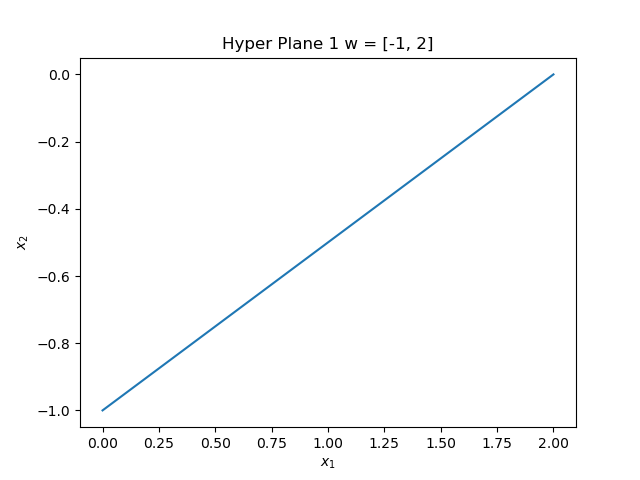
\includegraphics[width=10cm]{hyperplane1.png}
            \end{center}
            
        \subsubsection*{(A.9.b)}
            % plot it with python
            let $w = [1\quad 1\quad 1]^T, b = 20$, then the hyper plane $w^Tx + b = 0$ is implicit, explicitly we have the expression: 
            \begin{align*}\tag{1.9.b.1}\label{eqn:1.9.b.1}
                \begin{bmatrix}
                    1 \\ 1 \\ 1
                \end{bmatrix}^T 
                \begin{bmatrix}
                    x_1 \\ x_2 \\ x_3
                \end{bmatrix}
                + 0
                =&
                0
                \\
                x_1 + x_2 + x_3 =& 0
                \\
                x_3 =& -x_1 - x_2
            \end{align*}
            And we can just plot it.
            \begin{center}
                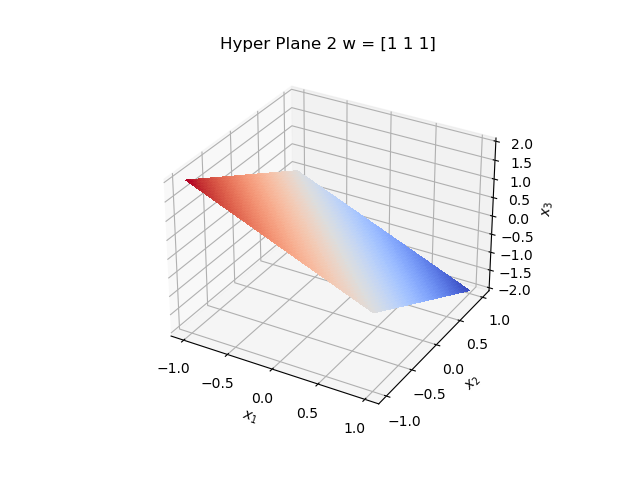
\includegraphics[width=10cm]{hyperplane2.png}
            \end{center}
            
        \subsubsection*{(A.9.c)}
            let $x^*$ be the optimal solution to the optimization problem, Using Lagrange Multiplier, the gradient of the objective and constraint gives us: 
            \begin{equation*}\tag{2.9.c.1}\label{eqn:2.9.c.1}
                \nabla_x[\left\Vert
                     x - x_0
                \right\Vert_2^2] = 2(x - x_0)
            \end{equation*}
            \begin{equation*}\tag{2.9.c.2}\label{eqn:2.9.c.2}
                \nabla_x[w^T + b] = w
            \end{equation*}
            Then we solve the system: 
            \begin{equation*}\tag{2.9.c.3}\label{eqn:2.9.c.3}
                \begin{cases}
                    2(x - x_0) = \lambda w
                    \\
                    w^Tx = -b
                \end{cases}
            \end{equation*}
            Let's solve the system together, we have: 
            \begin{align*}\tag{2.9.c.4}\label{eqn:2.9.c.4}
                x - x_0 =& \frac{\lambda}{2}w
                \\
                w^T(x - x_0) &= \frac{\lambda}{2}\Vert w\Vert_2^2
                \\
                -b - w^Tx_0 &= \frac{\lambda}{2}\Vert w\Vert_2^2
                \\
                \frac{\lambda}{2} &= \frac{-b - w^Tx_0}{\Vert w\Vert_2^2}
                \\
                \implies &
                \left\Vert
                     \frac{\lambda}{2} w
                \right\Vert_2
                = 
                \left\Vert
                    \frac{-b - w^Tx_0}{\Vert w\Vert_2^2} \frac{w}{\Vert w\Vert_2}
                \right\Vert_2
                =
                \left\vert
                     \frac{-b - w^Tx_0}{\Vert w\Vert_2}
                \right\vert
            \end{align*}
            The results is gotten, the same results can be gotten via the hint. 
    \subsection*{(A.10)}
        We define $f(x, y) = x^TAx + y^TBx + c$, and we are interested in the gradient of the function, derived from the ground up. 
        \subsubsection*{(A.10.a)}
            To express $f(x, y$ using summation notation, we first need to express $x^TAx$, which can be written as: 
            \begin{align*}\tag{2.10.a.1}\label{eqn:2.10.a.1}
                x^TAx =& x^T
                 \begin{bmatrix}  
                \sum_{j = 1}^n A_{1, j}x_j \\
                \sum_{j = 1}^n A_{2, j}x_j \\
                \vdots
                \\
                \sum_{j = 1}^n A_{n, j}x_j 
                \end{bmatrix}
                \\
                =& 
                \sum_{i = 1}^{n}x_i\left(
                    \sum_{j = 1}^{n}A_{i, j}x_j
                \right)
            \end{align*}
            By the same token, the expression for $y^TBx$ will look like: 
            \begin{equation*}\tag{2.10.a.2}\label{eqn:2.10.a.2}
                y^TBx = 
                \sum_{i = 1}^{n}y_i\left(
                    \sum_{j = 1}^{n}
                    B_{i, j}x_j
                \right)
            \end{equation*}
            Therefore, the whole function $f(x,y)$ can be written as: 
            \begin{align*}\tag{2.10.a.3}\label{eqn:2.10.a.3}
                f(x, y) =& x^TAx + y^TBx + c
                \\
                f(x, y) =& \sum_{i = 1}^{n}x_i\left(
                    \sum_{j = 1}^{n}A_{i, j}x_j
                \right) + 
                \sum_{i = 1}^{n}y_i\left(
                    \sum_{j = 1}^{n}
                    B_{i, j}x_j
                \right) + c
            \end{align*}
        \subsubsection*{(A.10.b)}
            To figure out the gradient of the function $f(x,y)$, we only need to focus on the $x^TAx$ part of the expression and then we play around with the indices when taking the derivative.
            \\
            First, let's choose an $x_k$ where $1 \le k \le n$ to take the partial derivative with, and then in the end we stack then vertically together and see what it is, let's get started by: 
            \begin{align*}\tag{2.10.b.1}\label{eqn:2.10.b.1}
                \partial_{x_k} \left[
                    \sum_{i = 1}^{n}x_i\left(
                        \sum_{j = 1}^{n}A_{i, j}x_j
                    \right)
                \right]
                =& 
                \sum_{i = 1}^{n}
                \partial_{x_k} \left[
                    x_i \sum_{j = 1}^{n}A_{i, j}x_j
                \right]
                \\
                =&
                \sum_{i = 1, i \neq k}^{n}
                \partial_{x_k} \left[
                    x_i
                        \sum_{j = 1}^{n}A_{i, j}x_j
                \right]
                +\partial_k \left[
                    x_k
                    \sum_{j = 1}^{n}A_{k, j}x_j
                \right]
                \\
                =&
                \sum_{i = 1, i \neq k}^{n}
                x_i
                \partial_{x_k} \left[ 
                        \sum_{j = 1}^{n}A_{i, j}x_j
                \right]
                +
                \sum_{j = 1}^{n}A_{k, j}x_j
                + 
                x_k
                \partial_k \left[
                    \sum_{j = 1}^{n}A_{k, j}x_j
                \right]
                \\
                =&
                \sum_{i = 1, i \neq k}^{n}
                \left(
                    x_i
                    A_{i, k}
                \right)
                + 
                \sum_{j = 1}^{n}A_{k, j}x_j
                + x_k A_{k, k}
                \\
                =&
                \sum_{i = 1}^{n}\left(x_i A_{i, k}\right)
                + 
                \sum_{j = 1}^{n}A_{k, j}x_j
            \end{align*}
            Cool, now we vertically stack the partial together to get the gradient for the function $f(x, y)$, which looks like: 

            \begin{align*}\tag{2.10.b.2}\label{eqn:2.10.b.2}
                \nabla_x[f(x, y)] = 
                \begin{bmatrix}
                    \sum_{i = 1}^{n}\left(x_i A_{i, 1}\right)
                    \\
                    \sum_{i = 1}^{n}\left(x_i A_{i, 2}\right)
                    \\
                    \vdots
                    \\
                    \sum_{i = 1}^{n}\left(x_i A_{i, n}\right)
                \end{bmatrix}
                +
                \begin{bmatrix}
                    \sum_{j = 1}^{n}A_{1, j}x_j\\
                    \sum_{j = 1}^{n}A_{2, j}x_j\\
                    \\
                    \vdots
                    \sum_{j = 1}^{n}A_{n, j}x_j
                \end{bmatrix}
                =
                A^Tx + Ax
            \end{align*}
        \subsubsection*{(A.10.c)}
            Now, taking derivative wrt to $y$ is way easier because we are dealing with a linear function wrt to the variable $y$, and we only need to focus on the term $y^TBx$, cause that is where the variable is at. Then taking the derivative will give us: 
            \begin{align*}\tag{2.10.c.1}\label{eqn:2.10.c.1}
                & \partial_{y_i} \left[
                    \sum_{i = 1}^{n}y_k
                        \sum_{j = 1}^{n}A_{i,j} x_j
                \right]
                \\
                =& 
                \partial_{y_k}
                y_k \sum_{j = 1}^{n}A_{k, j}x_j
                \\
                =&
                \sum_{j = 1}^{n}A_{k, j}x_j
            \end{align*}
            And it's not hard to see that, if we vertically stack the partial derivative together, we have $Ax$ to be $\nabla_y f(x, y)$.
    
            
\section*{3. Programming}
    \subsection*{A.11}
        \subsubsection*{(A.11.a), (A.11.b)}
        The results is output from the code, and I will use verbatim here: 
        \begin{verbatim}
    A^{-1} is:
    [[ 0.125 -0.625  0.75 ]
    [-0.25   0.75  -0.5  ]
    [ 0.375 -0.375  0.25 ]]
    Solved A{-1}b is:
    [[ 4.]
    [-3.]
    [ 1.]]
    Value for Ac is:
    [[6]
    [8]
    [7]]
        \end{verbatim}
    And here is the code that got me that result in python: 
\begin{lstlisting}[language=python]
# Plotings for HW0 
import numpy as np
import matplotlib.pyplot as plt
from matplotlib import cm
linspace = np.linspace
plot = plt.plot
savefig = plt.savefig
xlabel = plt.xlabel
ylabel = plt.ylabel
title = plt.title
meshgrid = np.meshgrid

def main(): 
    plotFirst()
    plotSecond()


def plotFirst():
    xs = linspace(0, 2, 1000)
    ys = xs/2 - 1
    plot(xs, ys)
    xlabel("$x_1$")
    ylabel("$x_2$")
    title("Hyper Plane 1 w = [-1, 2]")
    savefig("hyperplane1.png", format="png")


def plotSecond():
    fig, ax = plt.subplots(subplot_kw={"projection": "3d"})
    x = linspace(-1, 1, 1000)
    X, Y = meshgrid(x, x)
    Z = -X - Y
    _ = ax.plot_surface(X, Y, Z, cmap=cm.coolwarm, linewidth=0, antialiased=False)
    ax.set_zlim(-2, 2)
    ax.set_xlabel("$x_1$")
    ax.set_ylabel("$x_2$")
    ax.set_zlabel("$x_3$")
    ax.set_title("Hyper Plane 2 w = [1 1 1]")
    savefig("hyperplane2.png", format="png")

if __name__ == "__main__":
    import os
    print(f"cwd: {os.getcwd()}")
    print(f"curdir: {os.curdir}")
    main()


\end{lstlisting}
    \subsection*{A.12}
        \subsubsection*{(A.12.a)}
            Let's continue from \hyperref[eqn:1.6.c.2]{1.6.c.2}, where we derived that the variance of the random variable $\hat{F}_n(x) \le \frac{2}{4n}$, and apply it to here, we have: 
            \begin{equation*}\tag{A.12.a.1}\label{eqn:A.12.a.1}
                \text{Var}\left[\hat{F}_n(x)\right]
                    \le (0.0025)^2 = \frac{1}{4n}
            \end{equation*}
            An then we solve the equation $4n = \frac{1}{(0.0025)^2}$, which gives us: $n = 4000$, and that is the quantity we need. 
        \subsubsection*{(A.12.b)}
            For this part, we define a random variable to be like: 
            $$
                Y^{(k)} = \frac{1}{\sqrt{k}}\sum_{i = 1}^{n}
                    B_i
            $$
            Where, $B_i$ is a Bernoulli Distribution with $p = 0.5$, and now, we are making an empirical CDF for this random variable and plotting it. 
            \par
            So then we are essentially looking for the expected value of: 
            $$
                \hat{F}_n(x) = 
                \frac{1}{n}
                    \sum_{i = 1}^{n}
                        \mathbf{1}\{Y^{(k)}_i \le x\}
            $$

            And, each $Y_i^{k}$ is the same for all $i$. 
            \par
            To implement this, I created a function that creates empirical CDF functions given a generator for a random variable. 
            And here is the graph I have by the end: 
            \begin{center}
                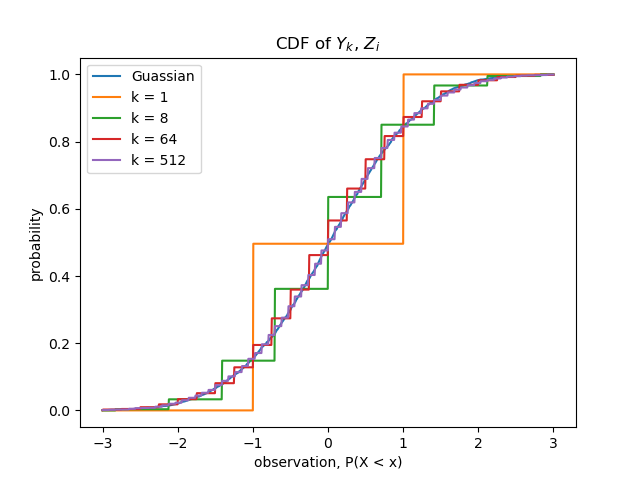
\includegraphics[width=10cm]{CDF.png}    
            \end{center}
            The code is implemented for part (b) is in \hyperref[lst:code]{here}. 
        \subsection*{All The codes Involved}
            \label{lst:code}\begin{lstlisting}[language=python]
## This is for the programming part of HW0 for class cse 546
import numpy as np
import matplotlib.pyplot as plt
inv = np.linalg.inv
solve = np.linalg.solve
rand = np.random.normal # Standard Gaussian
sum = np.sum
zeros = np.zeros
linspace = np.linspace
sqrt = np.sqrt

plot = plt.plot
show = plt.show
title = plt.title
xlabel = plt.xlabel
ylabel = plt.ylabel
legend = plt.legend
savefig = plt.savefig

A = np.array([[0, 2, 4], [2, 4, 2], [3, 3, 1]])
b = np.array([[-2], [-2], [4]])
c = np.array([[1], [1], [1]])


def A11a():
    print("A^{-1} is: ")
    print(inv(A))

def A11b():
    Solved = solve(A, b)
    print("Solved A{-1}b is: ")
    print(Solved)
    Ac = A@c
    print("Value for Ac is:")
    print(Ac)


def CDF(randomdVar:callable, xAxis, n:int=1000):
    """
        Given a random variable (PDF), this function will make a bounch of observation and
        look for the emprical CDF output, given the x-axis of course.

    :param ranomdVar:
        A function that return the random variable, and it should not have any argument.
    :param xAxis:
        The value you want to query the empirical CDF function
    :param n:
        The number of observations to make from the random variable.
    :return:
        The output of the empirical CDF function.
    """
    randomVarVec = np.vectorize(lambda x: randomdVar())
    Observations = randomVarVec(zeros(n))
    Observations = np.sort(Observations)
    Counter = 0
    Ys = zeros(xAxis.size)
    for II, x in np.ndenumerate(xAxis):
        while Counter < Observations.size and Observations[Counter] < x:
            Counter += 1
        Ys[II] = Counter
    return Ys/n


def A12a():
    """
        Take notice that the variance of the function hat(f)_n is what we want,
        this is shown in A.6 part (a).
        The sufficient value of n is:
    :return:
    """
    n = 4000
    Xs =  linspace(-3, 3, 1000)
    Z = lambda : rand(0, 1)
    Ys = CDF(randomdVar=Z, xAxis=Xs, n=n)
    plot(Xs, Ys)
    def Y(k):
        B = lambda: 1 if rand() < 0 else -1
        Bvec = np.vectorize(lambda x:B())
        y = Bvec(zeros(k))
        return sum(y)/sqrt(k)
    for k in [1, 8, 64, 512]:
        Ys = CDF(randomdVar=lambda :Y(k), xAxis=Xs, n=n)
        plot(Xs, Ys)
    title("CDF of $Y_k$, $Z_i$")
    xlabel("observation, P(X < x)")
    ylabel("probability")
    legend(["Guassian","k = 1", "k = 8", "k = 64", "k = 512"])
    show()
    savefig("CDF.png", format="png")


def main():
    A11a()
    A11b()
    A12a()

if __name__ == "__main__":
    import os
    print(f"current cwd: {os.getcwd()}")
    print(f"Cur dir {os.curdir}")
    main()
            \end{lstlisting}
         
\end{document}